\documentclass{standalone}
\usepackage{tikz}
\usetikzlibrary{hobby}

\begin{document}
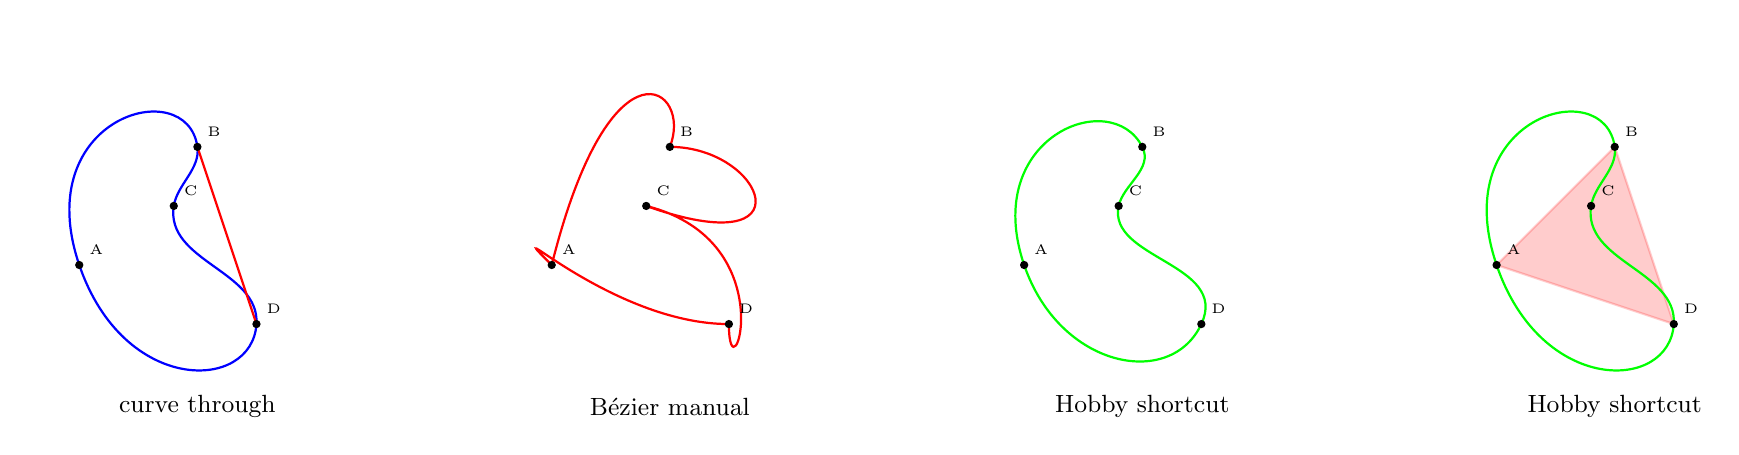
\begin{tikzpicture}[scale=1.5, every path/.style={thick}]
  % 1. curve through
  \begin{scope}[xshift=-4cm]
    \coordinate (A) at (0,0);
    \coordinate (B) at (1,1);
    \coordinate (C) at (0.8,0.5);
    \coordinate (D) at (1.5,-0.5);
    
    \draw[blue, closed] (A) to [curve through={(B) (C) }] (D);
    \draw [red] plot [smooth, tension=4] coordinates {(B) (D)};
    \node at (1, -1.2) {\small curve through};
    \foreach \pt in {A,B,C,D} {
      \fill (\pt) circle[radius=1pt];
      \node[font=\tiny, above right] at (\pt) {\pt};
    }
  \end{scope}

  % 2. manual Bezier
  \begin{scope}[xshift=0cm]
    \coordinate (A) at (0,0);
    \coordinate (B) at (1,1);
    \coordinate (C) at (0.8,0.5);
    \coordinate (D) at (1.5,-0.5);
    
    \draw[red]
      (A) .. controls (0.5,2) and (1.2,1.5) .. (B)
           .. controls (1.8,1) and (2.2,0) .. (C)
           .. controls (2,0.2) and (1.5,-1.2) .. (D)
           .. controls (0.5,-0.5) and (-0.5,0.5) .. (A);
    \node at (1, -1.2) {\small Bézier manual};
    \foreach \pt in {A,B,C,D} {
      \fill (\pt) circle[radius=1pt];
      \node[font=\tiny, above right] at (\pt) {\pt};
    }
  \end{scope}

  % 3. Hobby shortcut
  \begin{scope}[xshift=4cm]
    \coordinate (A) at (0,0);
    \coordinate (B) at (1,1);
    \coordinate (C) at (0.8,0.5);
    \coordinate (D) at (1.5,-0.5);
    
    \draw[green, use Hobby shortcut, closed]
      (A) .. (B) .. (C) .. (D);
    \node at (1, -1.2) {\small Hobby shortcut};
    \foreach \pt in {A,B,C,D} {
      \fill (\pt) circle[radius=1pt];
      \node[font=\tiny, above right] at (\pt) {\pt};
    }
  \end{scope}

  \begin{scope}[xshift=8cm]
    \coordinate (A) at (0,0);
    \coordinate (B) at (1,1);
    \coordinate (C) at (0.8,0.5);
    \coordinate (D) at (1.5,-0.5);
    
    % Convex hull: A-B-D (C is inside)
    \filldraw[red, opacity=0.2, draw=red]
      (A) -- (B) -- (D) -- cycle;
    
    % Smooth curve
    \draw[green, use Hobby shortcut, closed]
      (A) .. (B) .. (C) .. (D);
    
    \node at (1, -1.2) {\small Hobby shortcut};
    \foreach \pt in {A,B,C,D} {
      \fill (\pt) circle[radius=1pt];
      \node[font=\tiny, above right] at (\pt) {\pt};
    }
  \end{scope}
\end{tikzpicture}
\end{document}
